\chapter{Structures de données classiques}
\section{\texttt{Pile}}
	\subsection{Statique}
	Cf exemple de cours section \ref{pileStatique} page \pageref{pileStatique}, une amélioration est également présente ci-dessous.
\begin{enumerate}
	\item Implémenter la fonction permettant de remplacer toute les occurrences de l'élément x par l'élément y dans la pile.
	\item Implémenter la fonction d'affichage de la Pile.
	\item Réécrire les méthode de la pile statique pour prendre en compte la protection du type
\end{enumerate}
\begin{description}
	\item[Rajouter dans le champ des opérations] \texttt{remplacerOccurence} Pile $\times$ Element $\times$ Element $\rightarrow$ Pile
	\item[Préconditions] rien
	\item[Axiones]
\end{description}

\begin{lstlisting}[language=C]
remplacerOccurence(creer(), x, y) = creer();
remplacerOccurence(empiler(p, x), x1, x2) = 
		p1 $\wedge$ $\forall z$ (appartient(p1, z) $\rightarrow$ (z $\neq$ x1) (empiler(p, x), z') $\wedge$ z' = x1))
\end{lstlisting}
\lstinputlisting[language=C, caption=TAD Pile]{annexes/exercices/1.c}
\section{\texttt{Dynamique}}
\lstinputlisting[language=C, caption=TAD Pile]{content/pileDynamique.c}
\lstinputlisting[language=C, caption=TAD Pile]{content/pileDynamique.h}

\section{\texttt{File}}
\begin{description}
	\item[Sorte] File
	\item[Utilise] Element, booleen
	\item[Constructeurs]~
		\begin{description}
			\item[\texttt{creer}] $\rightarrow$ File% CONSTRUCTEURS
			\item[\texttt{enfiler}] \texttt{File} $\times$ Element $\rightarrow$ File
		\end{description}
	\item[Projecteurs] 
		\begin{description}
			\item[\texttt{estVide}] file $\rightarrow$ Booleen
			\item[\texttt{appartient}] file $\times$ Element $\rightarrow$ Booleen
			\item[\texttt{defiler}] file $\rightarrow$ file
			\item[\texttt{premier}] file $\rightarrow$ Element
			\item[\texttt{dernier}] file $\rightarrow$ Element
		\end{description}
	\item[Précondition]~
		\begin{description}
			\item[\texttt{premier}] premier(f) $\Leftrightarrow$ $\neg$estVide(f) 
			\item[\texttt{dernier}] dernier(f) $\Leftrightarrow$ $\neg$estVide(f) 
		\end{description}
	\item[Axiones]~
\begin{lstlisting}[language=C, numbers=none,caption=Axiones du TAD File]
estVide(creer()) = true;
estVide(enfiler(f,x)) = false;
appartient(creer(), x) = false;
appartient(enfiler(f,x),y) = (x = y) $\vee$ appartient(f,y)
defiler(creer()) = creer()
defiler(enfiler(f,x) = creer() si estVide(f)
					 = enfiler(defiler(f), x) sinon
premier(enfiler(f,x)) = premier(f) si !estVide
					  = x sinon
dernier(enfiler(f,x)) = x
\end{lstlisting}
\end{description}
	\subsection{Statique}
\lstinputlisting[language=C, caption=TAD File dynamique Headers]{annexes/exercices/3.h}
\lstinputlisting[language=C, caption=TAD File dynamique Implémentation]{annexes/exercices/3.c}
	\subsection{Dynamique}
\lstinputlisting[language=C, caption=TAD File dynamique Headers]{annexes/exercices/4.h}
\lstinputlisting[language=C, caption=TAD File dynamique Implémentation]{annexes/exercices/4.c}

\subsubsection{Application de la \texttt{File} à la fusion de voies routières}
\paragraph{Amélioration de la \texttt{File} en dynamique} Ecrire dans le module \texttt{File} (en dynamique) les deux fonctions suivantes : 
\begin{itemize}
	\item \texttt{concat}: \texttt{File} $\times$ \texttt{File} $\rightarrow$ \texttt{File}
	\item \texttt{mixe}: \texttt{File} $\times$ \texttt{File} $\rightarrow$ \texttt{File}
\end{itemize} ~

\lstinputlisting[language=C, caption=TAD File dynamique Implémentation \texttt{concat} et \texttt{mixe}]{annexes/exercices/4-1.c}
\paragraph{Écrire l'application} ~
\lstinputlisting[language=C, caption=Application de fusion de voies routières]{annexes/exercices/4-2.c}
\section{\texttt{File} avec priorité}
Ce sont des files dans lesquelles on place chaque élément au <<bon endroit>> (en remplaçant les priorités).

On va considérer qu'il existe dans le module \texttt{Element}, une fonction qui permet de comparer deux éléments entre eux.
\begin{lstlisting}[language=C, numbers=none,caption=Fonction comparer]
/*
 * Renvoie   0 si e1 et e2 sont de même priorité
 *			-1 si e1 est moins prioritaire que e2
 *           1 si e1 est plus prioritaire que e2
 */
int compare(elem e1, elem e2);
\end{lstlisting}
\attention{Le main de la fonction pourrait changer suivant les éléments}
Réécrire enfiler en utilisant un pointeur de fonction pour accéder à la fonction de comparaison.
\section{\texttt{Liste} avec priorité}
Nous allons utiliser une liste doublement chaînée.
\begin{figure}[H]
	\centering
\includegraphics[width=12cm]{content/fileDoubleChaine.eps}
	\caption{Liste doublement chaînée}
\end{figure}

\begin{enumerate}
	\item Proposer un type C pour la liste doublement chainée
	\item \'Ecrire les méthodes suivantes:  \\
\begin{lstlisting}[language=C, numbers=none]
LDC creer();
LDC ajouter(LDC, Elem);
void affichageCroisant(LDC);
void afficheDecroissant(LDC);
LDC supprimer(LDC, Elem);
/* Application de la fonction à chaqcun des éléments de la LDC et renvoie
 * la LDC des résultats 
 */
LDC map(fonction, LDC) 
\end{lstlisting}
\end{enumerate}
\lstinputlisting[language=C, caption=Header liste doublement chainée]{annexes/exercices/5.h}
\lstinputlisting[language=C, caption=Source lite doublement chainée]{annexes/exercices/5.c}
